\paragraph{Tổ chức các hàm và ranh giới transaction.}
\label{sec:inventory-implementation}
\begin{longtable}{|p{.33\linewidth}|p{.58\linewidth}|}
\hline\textbf{Hàm/thành phần} & \textbf{Trách nhiệm}\\\hline\endhead
OrdersService.create & Xác lập quyền sở hữu idempotency key, tính giá/voucher, gọi reserve, tạo Order/OrderItem/snapshot và gắn kết quả vào key trong một transaction.\\\hline
ingredientDemand & Chuyển lựa chọn món/size/topping thành tổng lượng theo ingredientId; kiểm tra định lượng và giới hạn số nguyên.\\\hline
InventoryService.reserve & Đọc công thức, tính demand, khóa Ingredient theo id tăng dần, kiểm đủ toàn bộ rồi trừ; trả lượng đã trừ để lưu snapshot.\\\hline
OrdersService.cancel & Kiểm tra quyền/trạng thái, khóa Order, kiểm tra thanh toán, cập nhật CANCELLED có điều kiện và gọi release.\\\hline
InventoryService.release & Khóa snapshot theo đơn; chặn thiếu snapshot/đã hoàn; cộng lại quantity và ghi releasedAt trong transaction do hàm gọi cung cấp.\\\hline
ReservationExpiryService & Tìm đơn quá hạn đủ điều kiện, lấy khóa không chờ trên đơn, kiểm lại sau khóa, release và đóng đơn; phát thông báo sau commit.\\\hline
ExchangeService.decide & Khi duyệt đổi, khóa Order cũ và tập nguyên liệu liên quan, hoàn snapshot cũ, giữ lựa chọn mới và tạo đơn thay thế trong cùng transaction.\\\hline
\caption{Phân trách nhiệm để tái sử dụng và kiểm thử độc lập}
\end{longtable}

\paragraph{Tính nguyên tử.}
Giả sử đơn có cà phê và trà: cà phê còn đủ nhưng trà hết. Backend không được tạo một nửa Order hoặc giữ riêng phần cà phê. Transaction làm cho thao tác hoặc commit toàn bộ hoặc rollback toàn bộ. Tương tự, hủy đơn không được commit trạng thái CANCELLED nhưng bỏ quên bước hoàn nguyên liệu. Snapshot, kho và trạng thái phải cùng commit.

\paragraph{Chống gửi lặp trước khi chạm kho.}
Unique key theo khách trong OrderCreateRequest được xác lập trước reserve. Hai request cùng key cùng nội dung sẽ quy về một Order; key cũ với nội dung khác bị từ chối. Vô hiệu hóa nút frontend chỉ hỗ trợ thao tác, còn ràng buộc database mới bảo vệ khi request bị gửi lại hoặc có nhiều tab/process. Khi một transaction tranh key thất bại, backend rollback rồi đọc kết quả đã lưu, không tiếp tục truy vấn trong transaction đang lỗi.

\paragraph{Chống tranh phần cuối bằng khóa dòng.}
Reserve dùng SELECT FOR UPDATE trên các Ingredient cần dùng. Nếu A và B cùng cần 20g cuối, A lấy khóa trước, kiểm đủ rồi trừ về 0 và commit. B chờ khóa; khi được xử lý, B thấy tồn 0 nên bị từ chối. Khóa chỉ giữ trong transaction ngắn; không giữ trong lúc khách chọn món hoặc mở trang VNPay. Database còn có CHECK stock không âm như lớp bảo vệ dữ liệu.

Khóa theo id tăng dần giúp các transaction lấy nhiều nguyên liệu theo cùng thứ tự. Ví dụ cả A và B đều lấy nguyên liệu 1 rồi 2, tránh tình huống mỗi bên giữ một nguyên liệu rồi chờ nguyên liệu của bên kia. Các luồng thanh toán/hủy/hết hạn cùng lấy khóa Order trước để kiểm tra trạng thái nhất quán.

\paragraph{Hoàn đúng một lần.}
Hai yêu cầu hủy cùng Order phải qua khóa Order và cập nhật trạng thái có điều kiện. Chỉ giao dịch thực sự chuyển được trạng thái mới release. Bên trong release, snapshot tiếp tục được khóa và releasedAt được kiểm tra. Hai lớp này bảo vệ cả API hủy lẫn việc gọi lại hàm release; lỗi sau khi cộng kho vẫn rollback cả dấu hoàn.

\paragraph{Nhiều worker và thông báo.}
Cờ running tránh hai lượt quét chồng trong một process. SELECT FOR UPDATE SKIP LOCKED mới là cơ chế phối hợp ở database khi nhiều worker cùng xử lý một đơn: bên chưa lấy được khóa bỏ qua, không xử lý trùng. Sau khi lấy khóa, worker đọc lại trạng thái và bằng chứng nhận tiền. Thông báo orders.changed phát sau commit; UI tải lại dữ liệu và có polling HTTP 15 giây khi tab hiển thị. Tác vụ quét tiếp tục khi backend khởi động lại vì deadline nằm trong database.

\paragraph{Kết hợp khóa dòng và kiểm tra phiên bản.}
Kho và vòng đời Order dùng khóa dòng. OrderExchange và PaymentRefundCase dùng thêm cập nhật có điều kiện theo version: chỉ ghi khi id/version/trạng thái còn khớp, rồi tăng version; cập nhật không tác động một dòng trả lỗi xung đột. Ví dụ hai barista cùng đọc version=0 thì người ghi sau không thể ghi đè quyết định đã nâng lên version=1. Mỗi cơ chế gắn với đối tượng nghiệp vụ cụ thể.

\begin{figure}[p]\centering
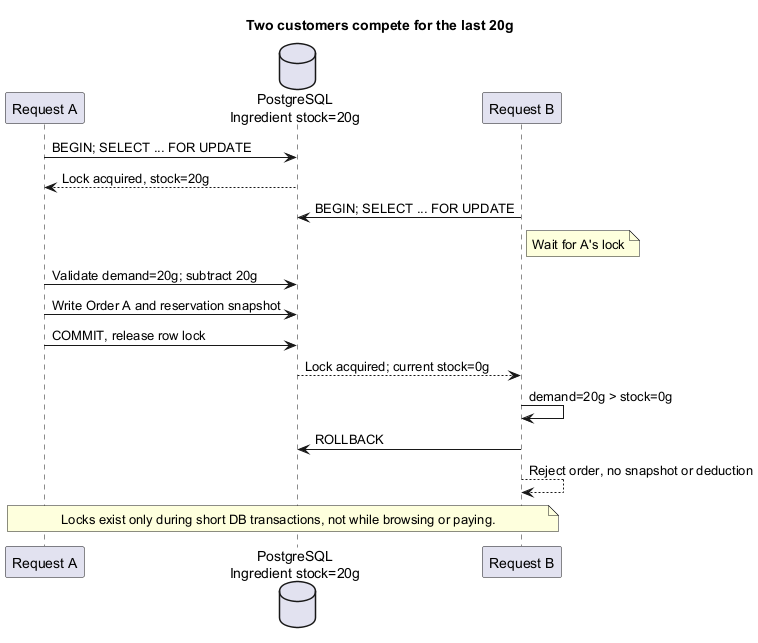
\includegraphics[width=\linewidth,height=.78\textheight,keepaspectratio]{assets/inventory/inventory-concurrency.png}
\caption{Hai khách tranh phần nguyên liệu cuối: chỉ transaction đủ kho được commit}
\end{figure}

\paragraph{Ảnh chụp code từ phiên bản hiện thực.}
Các hình sau được chụp từ mã nguồn hiện tại; tên tệp và số dòng nằm trên ảnh để truy vết. Phần giải thích đọc cùng các hàm gọi bên ngoài: reserve/release nhận TransactionClient, nên ranh giới commit/rollback do service gọi quản lý.

\begin{figure}[p]\centering
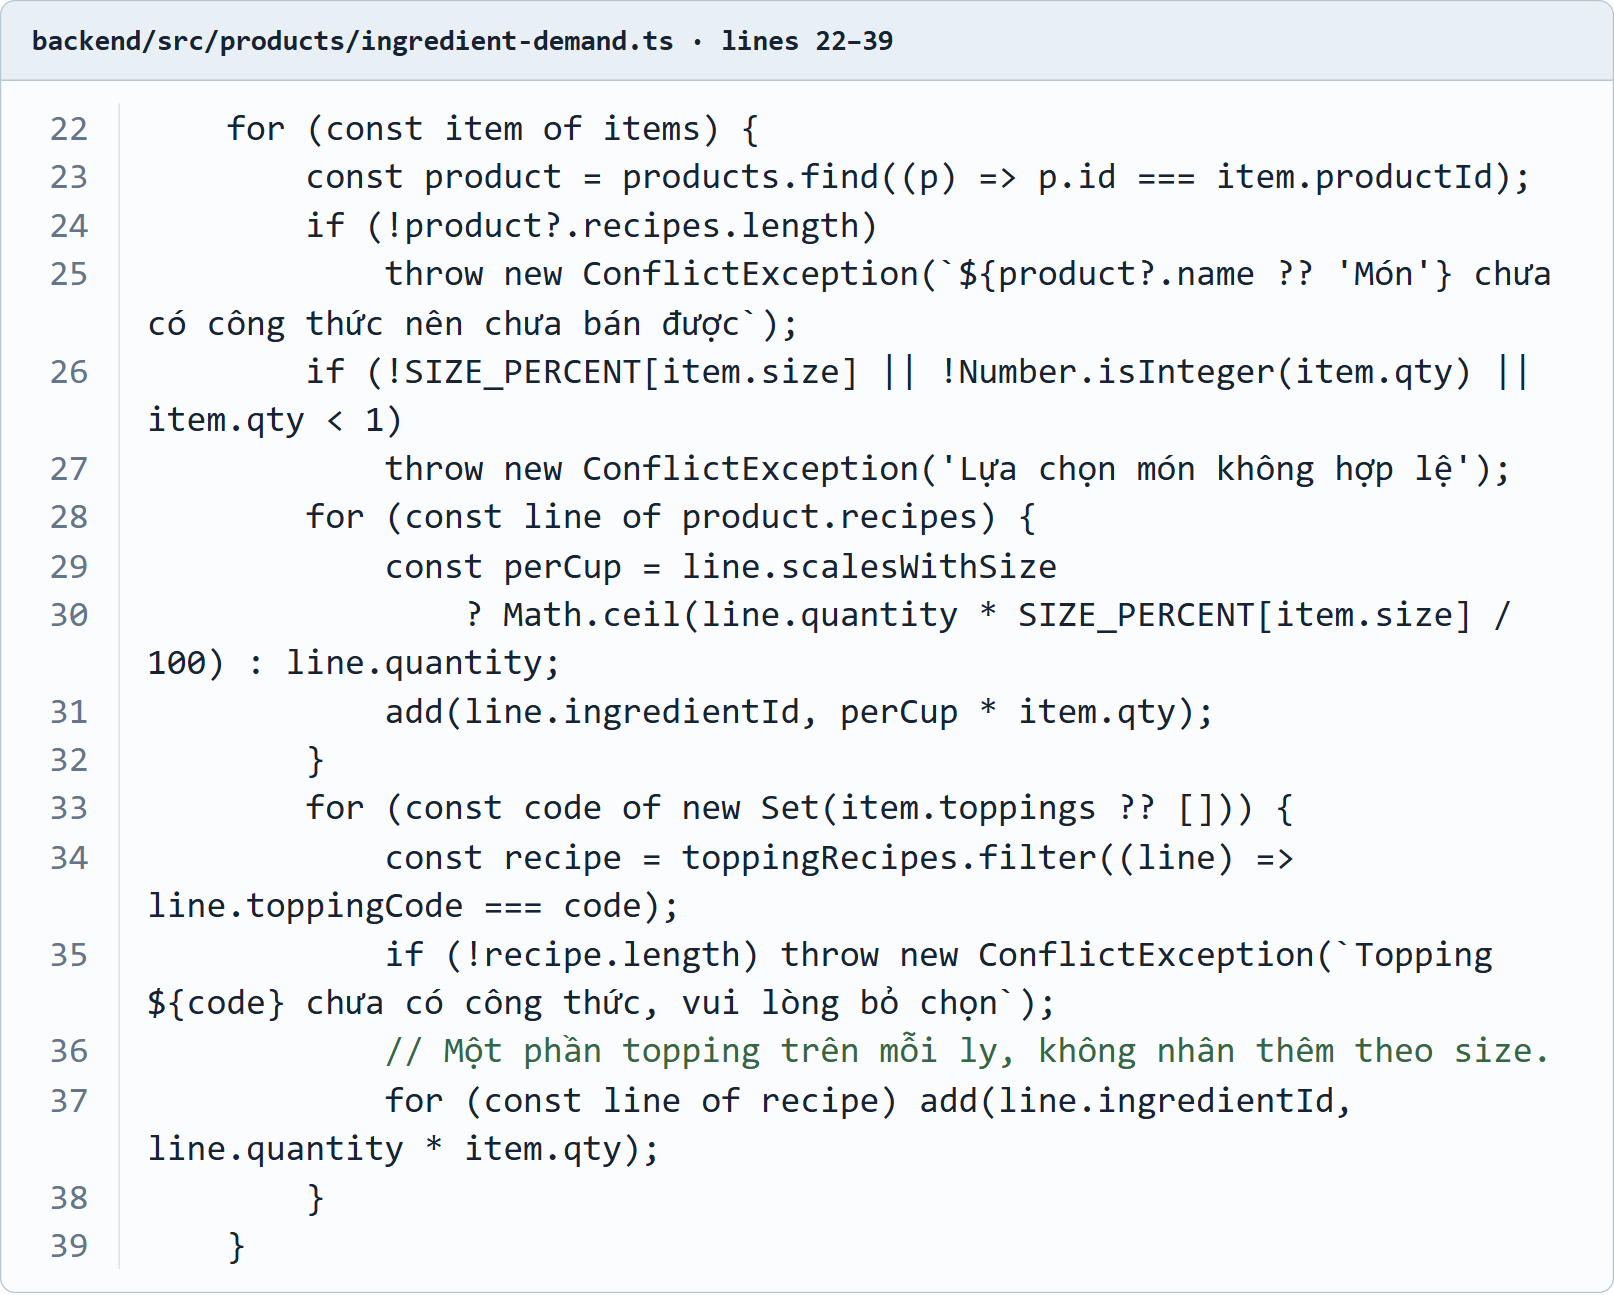
\includegraphics[width=\linewidth,height=.79\textheight,keepaspectratio]{assets/inventory/code-demand.png}
\caption{ingredientDemand: tính size, vật tư cố định, topping và cộng gộp nguyên liệu}
\end{figure}
\clearpage
\begin{figure}[p]\centering
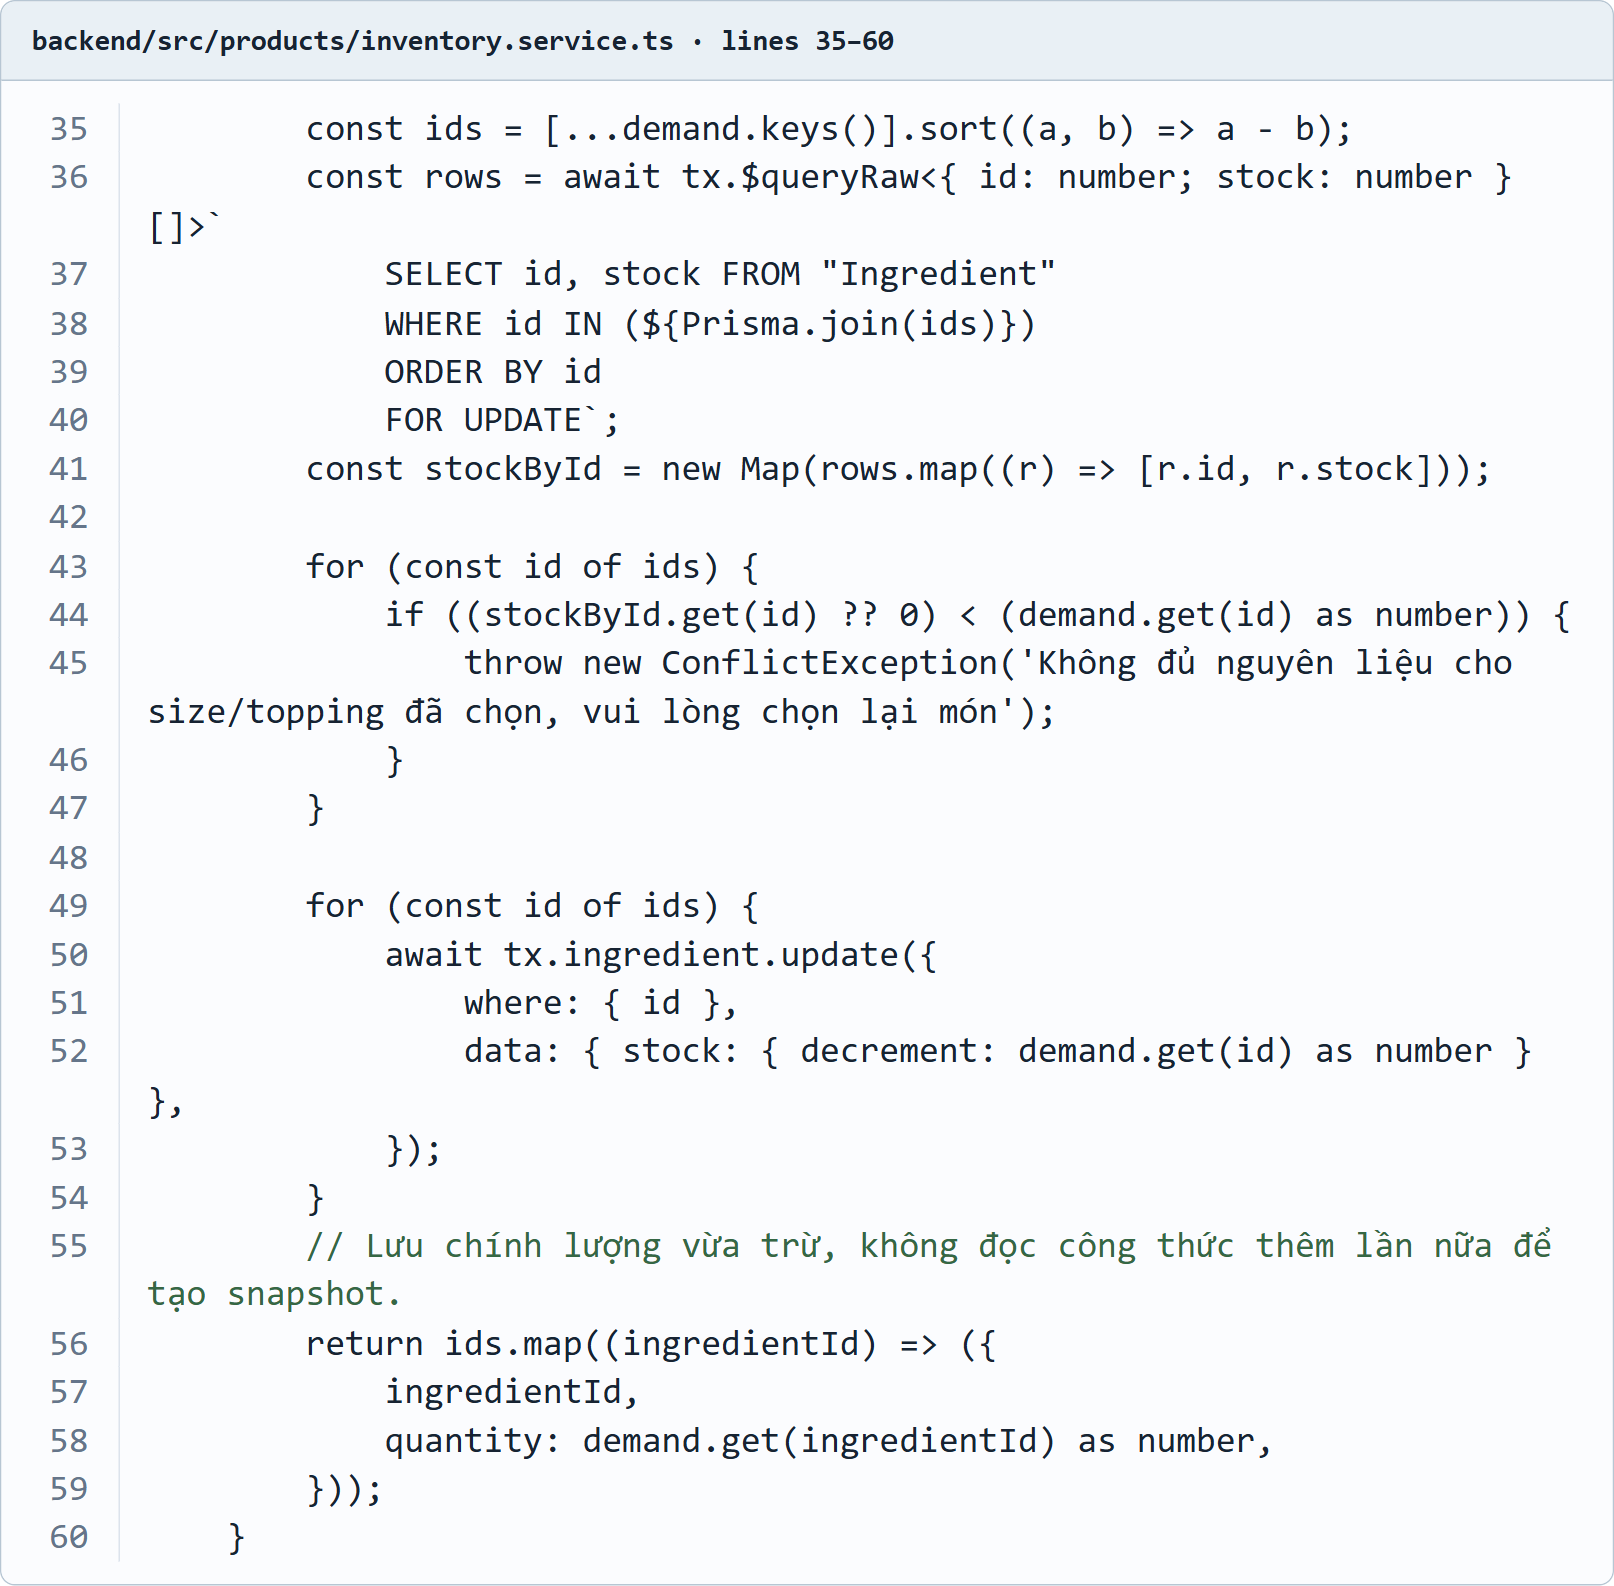
\includegraphics[width=\linewidth,height=.79\textheight,keepaspectratio]{assets/inventory/code-reserve.png}
\caption{reserve: khóa dòng theo thứ tự id, kiểm kho, trừ và trả snapshot}
\end{figure}
\clearpage
\begin{figure}[p]\centering
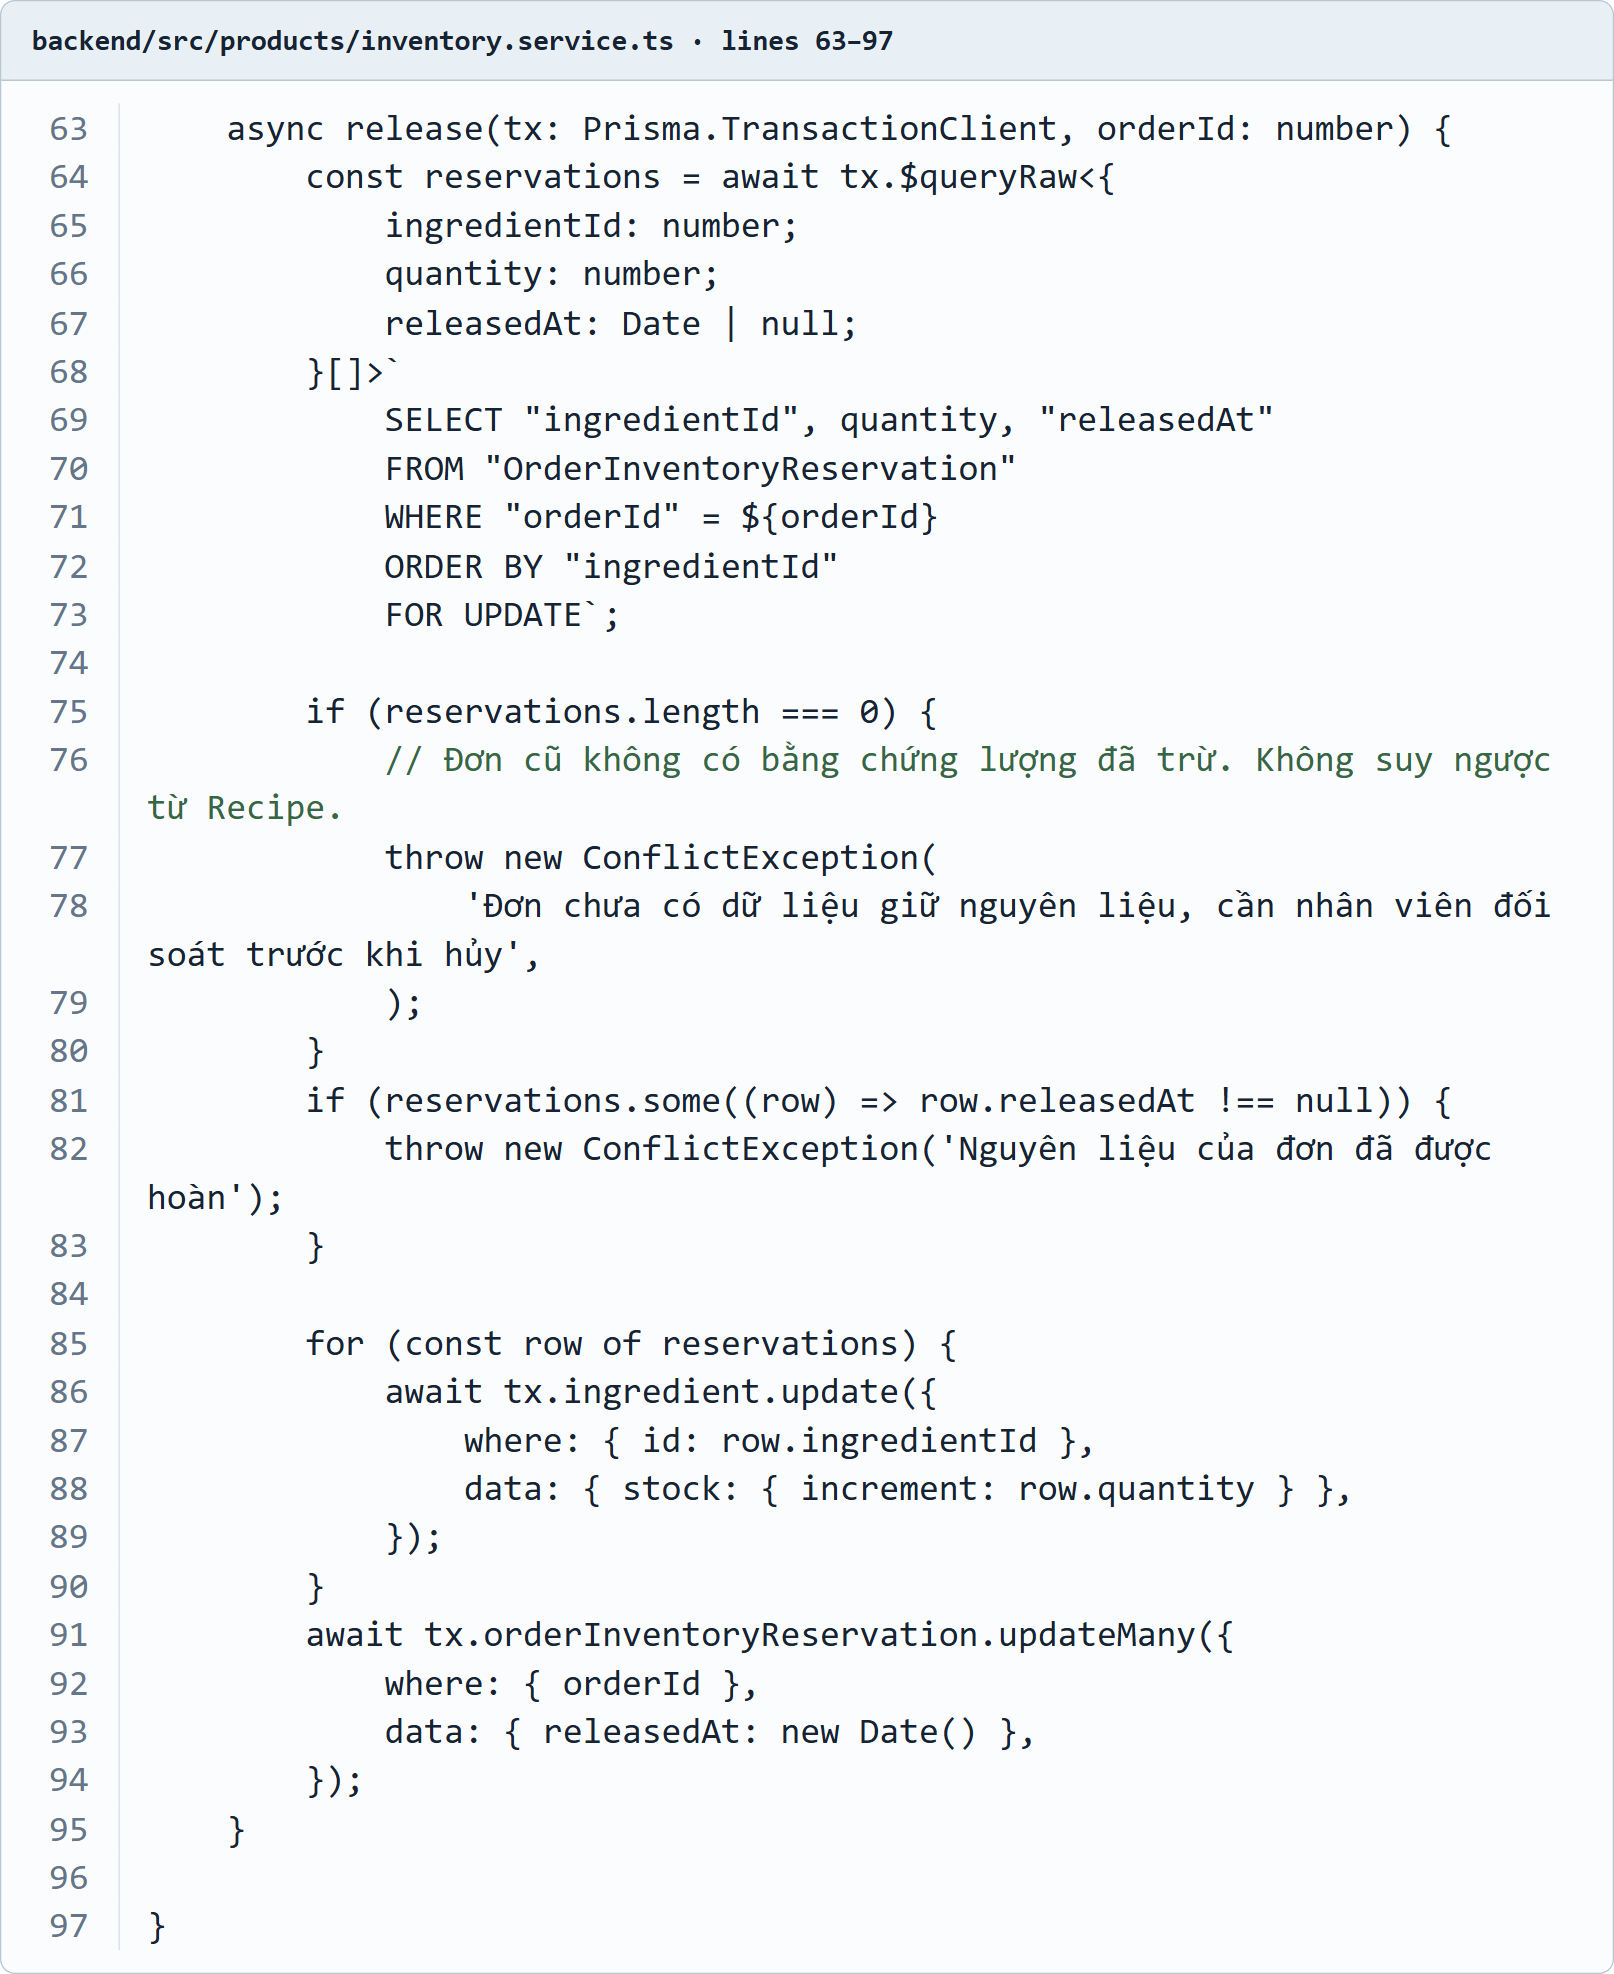
\includegraphics[width=\linewidth,height=.79\textheight,keepaspectratio]{assets/inventory/code-release.png}
\caption{release: khóa snapshot, chặn hoàn lại và cộng đúng lượng lịch sử}
\end{figure}
\clearpage
\begin{figure}[p]\centering
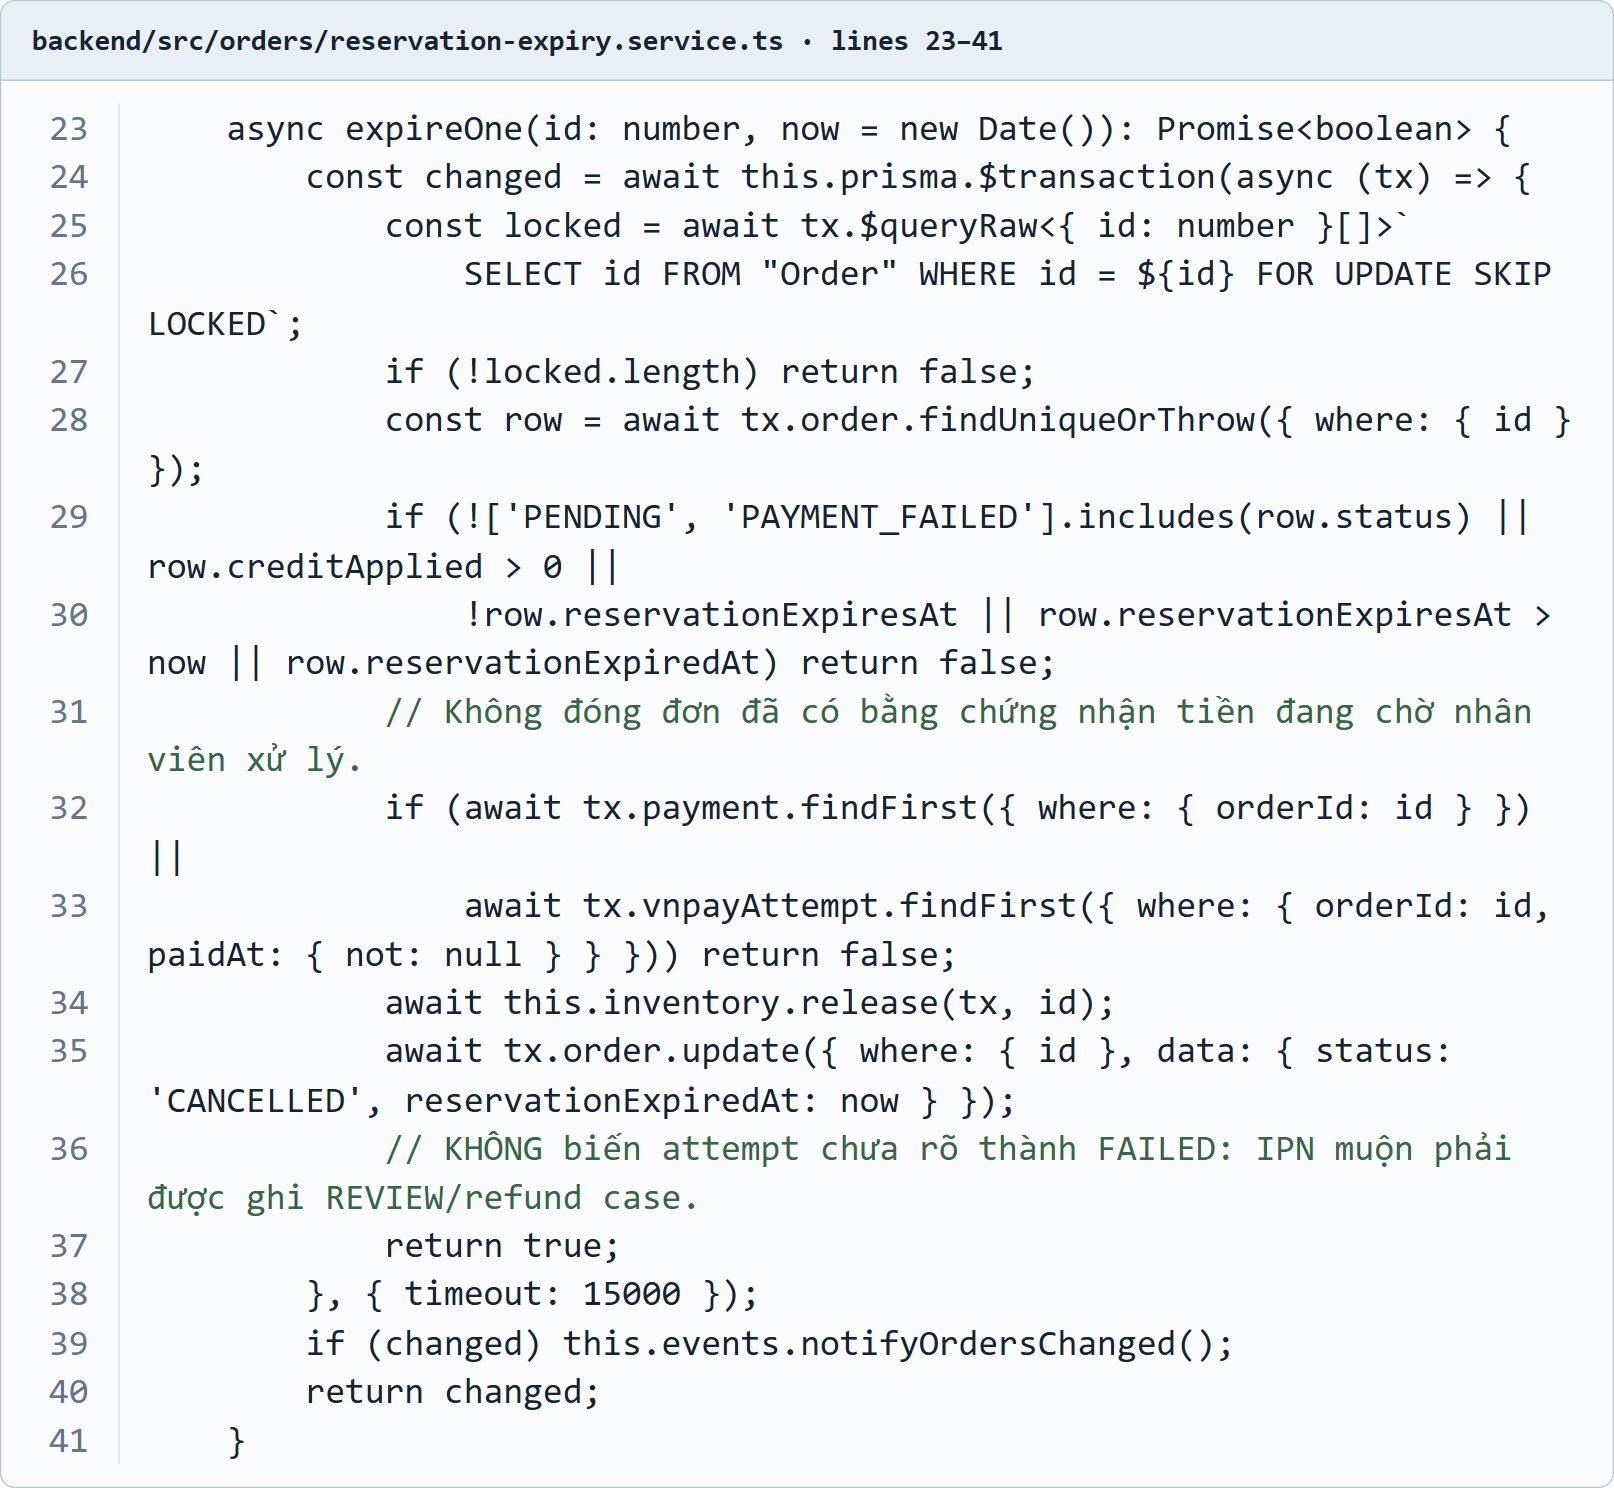
\includegraphics[width=\linewidth,height=.79\textheight,keepaspectratio]{assets/inventory/code-expiry.png}
\caption{expireOne: phối hợp worker, kiểm tra bằng chứng thanh toán và đóng đơn nguyên tử}
\end{figure}
\clearpage
